\section{Scheduler Modifications}

With the above scheduling flow control in mind, we sought out to change and tune the CFS system in some meaningful way. Among the many traits a scheduler is desired to exhibit, we decided to modify the scheduler to measure and tweak it's throughput, scheduling period, and individual process runtime. These tests were not necessarily designed to improve the kernel, but rather to explicitly test how various properties affect it's performance. There were three main source modifications we attempted:
\begin{enumerate}
	\item Modify the logic behind which process is chosen in \texttt{pick\_next\_entity()}
	\item Change the kernel parameters at runtime to cause frequent context switching
	\item Modify CFS bandwidth and quota to cause artificial throttling
\end{enumerate}

\vspace{1pc}
\noindent\textbf{1 Picking Next Entity Changes}

\vspace{1pc}

The first and most simplistic change involved modifying the operation of \texttt{pick\_next\_entity()} in fair.c. As mentioned above, this function is the last authority queried in the scheduling flow control of CFS, which means process traffic can be changed here. A simplified psudocode version of \texttt{pick\_next\_entity()} is as follows:
\begin{lstlisting}
pick_next_entity(cfs_rq, currentProcess)

SchedulerEntity left = PickFirstEntity()
SchedulerEntity se

if (currentProcess is left of leftmost entity)
	left = currentProcess

se = left

if (cfs_rq->skip should skip se){
	//skip buddy
}

if (cfs_rq->last and WakeupPreemptEntity())
	se = cfs_rq->last
	
if (cfs_rq->next and WakeupPreemptEntity())
	se = cfs_rq->next

return se
\end{lstlisting}

By removing the additional logic from lines 11-19, we can force the cfs scheduler to strictly run the leftmost (most needed) entity from the red-black tree, and bypass the additional logic used to make exceptions. The resulting psudocode is as follows:

\begin{lstlisting}
pick_next_entity(cfs_rq, currentProcess)

SchedulerEntity left = PickFirstEntity()
SchedulerEntity se

if (currentProcess is left of leftmost entity)
	left = currentProcess

se = left

return se
\end{lstlisting}

\vspace{1pc}

\noindent\textbf{2 Changing Kernel Parameters}
\vspace{1pc}

Changing kernel parameters is not terribly difficult and can be done fairly easily from several different source files before compilation. Areas of focus include the targeted preemption latency and minimum preemption granularity in fair.c, min/max priority niceness values in prio.h, \texttt{SCHED\_LOAD\_SCALE} (which adjusts the number of shares available for the root group) and \texttt{RUNTIME\_INF} for cfs\_rq quota in sched.h. (landley.com)

Some kernel parameters have the benefit of being publically readable and  writable during runtime. The utility \texttt{sysctl} can be used to read and write to kernel parameters at runtime, changing the behavior of everything from average Round Robin time slicing to CFS bandwidth.

Additionally, many kernel parameters can be read from the /proc folder, providing a secondary resource for details on cgroups, hardware info and process specific information.

\begin{figure}[hb]
	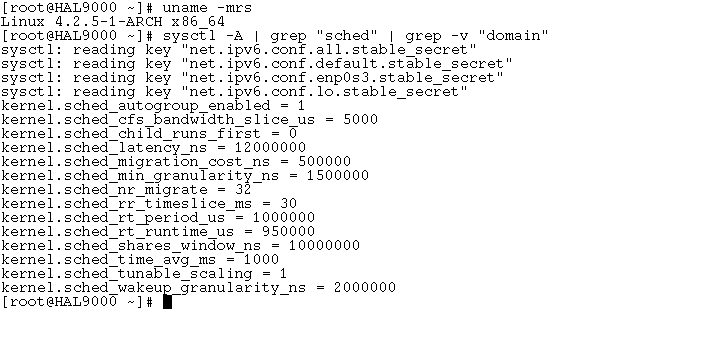
\includegraphics[width=1.0\columnwidth]{images/sysctl}
	\caption{Displaying the default values for the stock Arch Linux Kernel}
\end{figure}

\vspace{1pc}

\noindent\textbf{3 CFS Bandwidth and Quota}

\vspace{1pc}

As it turns out, the Linux scheduling system makes use of time in any way it possibly can. Additionally, it can also be made to limit or even restrict certain groups of processes from using 100\% of cpu resources at all times. These features are made possible through several parameters:
\begin{description}
	\item [rt\_period\_us] represents the bandwidth enforcement interval in microseconds (default is 100000000us)
	\item [rt\_runtime\_us] represents the permitted amount of rt\_period\_us that may be used during a given period (default is 95000000us)
	\item [runtime\_inf] changes the default quota assigned to CFS (default value is disabled, meaning that CFS has unconstrained use of the cpu)
\end{description}

(blaess)(landley)